%! Author = melek
%! Date = 9.06.2022

% Preamble
\documentclass[11pt]{article}

% Packages
\usepackage{amsmath}
\DeclareMathOperator*{\argmax}{argmax}

\usepackage{graphicx}
\usepackage{amssymb}
\usepackage{bm}

\graphicspath{ {../images/} }


% Document
\begin{document}

    \maketitle
    \setcounter{section}{11}


    \section{Exercises}

    \subsection{Question}

    Just as the return can be written recursively in terms of the first reward and itself one-step later (3.9), so can the $\lambda$-return.
    Derive the analogous recursive relationship from (12.2) and (12.1).

    \subsection*{Answer}

    \noindent Equation 12.1:

    \noindent $ G_{t_t+n} = R_{t+1} + \gamma R_{t+2}+ \gamma^2 R_{t+3} + \ldots + \gamma^{n-1} R_{t+n} + \gamma^n \hat{v}(S_{t+n}, w_{t+n-1}) $

    \noindent Equation 12.2:

    \noindent $ G_{t}^\lambda = (1-\lambda) \sum_{n=1}^{\infty} \lambda^{n-1} G_{t:t+n} $

    \hfill \break
    \noindent Let's start with expanding 12.2:

    \noindent $ G_{t}^\lambda = (1-\lambda) [ \lambda^{0} G_{t:t+1} + \lambda^{1} G_{t:t+2} + \lambda^{2} G_{t:t+3} + \ldots ] $

    \noindent $ G_{t}^\lambda = (1-\lambda) G_{t:t+1} + (1-\lambda) [ \lambda^{1} G_{t:t+2} + \lambda^{2} G_{t:t+3} + \ldots ] $

    \noindent $ G_{t}^\lambda = (1-\lambda) G_{t:t+1} +  \lambda (1-\lambda)  [ \lambda^{0} G_{t:t+2} + \lambda^{1} G_{t:t+3} + \ldots ] $

    \noindent $ G_{t}^\lambda = (1-\lambda) G_{t:t+1} +  \lambda (1-\lambda) \sum_{n=1}^{\infty} \lambda^{n-1} G_{t:t+1+n} $

    \hfill \break
    \noindent Let's not touch the left expression for now and focus on the second expression.
    We have a return of form $ G_{t:t+1+n} $ but a return of form $ G_{t+1:t+1+n} $ would be more useful.
    Let's try to express one in the form of the other.

    \noindent $ G_{t+1:t+1+n} =  R_{t+2} + \gamma R_{t+3} + \ldots + \gamma^{n-1} R_{t+1+n} + \gamma^n \hat{v}(s_{t+1+n},w_{t+n})  $ (12.1.1)

    \noindent $ G_{t:t+1+n} =  R_{t+1} + \gamma R_{t+2} + \gamma^2 R_{t+3} + \ldots + \gamma^{n} R_{t+1+n} + \gamma^{n+1} \hat{v}(s_{t+1+n},w_{t+n})  $

    \noindent $ G_{t:t+1+n} =  R_{t+1} + \gamma [R_{t+2} + \gamma R_{t+3} + \ldots + \gamma^{n-1} R_{t+1+n} + \gamma^{n} \hat{v}(s_{t+1+n},w_{t+n})]  $

    \noindent $ G_{t:t+1+n} =  R_{t+1} + \gamma G_{t+1:t+1+n}  $ (12.1.2)

    \hfill \break
    \noindent Going back and using equation (12.1.2):

    \noindent $ G_{t}^\lambda = (1-\lambda) G_{t:t+1} +  \lambda (1-\lambda) \sum_{n=1}^{\infty} \lambda^{n-1} (R_{t+1} + \gamma G_{t+1:t+1+n}) $

    \noindent $ G_{t}^\lambda = (1-\lambda) G_{t:t+1} +  \lambda (1-\lambda) \sum_{n=1}^{\infty} \lambda^{n-1} R_{t+1 }+   \lambda (1-\lambda) \sum_{n=1}^{\infty} \lambda^{n-1} \gamma G_{t+1:t+1+n} $

    \noindent $ G_{t}^\lambda = (1-\lambda) G_{t:t+1} +  \lambda (1-\lambda) \sum_{n=1}^{\infty} \lambda^{n-1} R_{t+1 }+   \gamma \lambda (1-\lambda) \sum_{n=1}^{\infty} \lambda^{n-1}  G_{t+1:t+1+n} $

    \hfill \break
    \noindent We have a geometric series of form $ ( \sum_{n=1}^{\inf} r \lambda^{n-1} = \frac{r}{1-\lambda} ) $:

    \noindent $ G_{t}^\lambda = (1-\lambda) G_{t:t+1} +  \lambda (1-\lambda)  \frac{R_{t+1}}{(1-\lambda)} +  \gamma \lambda (1-\lambda) \sum_{n=1}^{\infty} \lambda^{n-1} G_{t+1:t+1+n} $

    \noindent $ G_{t}^\lambda = (1-\lambda) G_{t:t+1} +  \lambda R_{t+1} +  \gamma \lambda (1-\lambda) \sum_{n=1}^{\infty} \lambda^{n-1} G_{t+1:t+1+n} $

    \hfill \break
    \noindent The right most expression is a lambda return:

    \noindent $ G_{t}^\lambda = (1-\lambda) G_{t:t+1} +  \lambda R_{t+1} +  \gamma \lambda G_{t+1}^\lambda $

    \hfill \break
    \noindent We can further simplify by expanding the 1-step return:

    \noindent $ G_{t}^\lambda = (1-\lambda) (R_{t+1} + \gamma G_{t+1:t+1}) +  \lambda R_{t+1} +  \gamma \lambda G_{t+1}^\lambda $

    \noindent $ G_{t}^\lambda = (1-\lambda) (R_{t+1} + \gamma \hat{v}(s_{t+1},w_{t}) ) +  \lambda R_{t+1} +  \gamma \lambda G_{t+1}^\lambda $

    \noindent $ G_{t}^\lambda = (1-\lambda) \gamma \hat{v}(s_{t+1},w_{t})  + (1-\lambda) R_{t+1} +  \lambda R_{t+1} +  \gamma \lambda G_{t+1}^\lambda $

    \noindent $ G_{t}^\lambda = (1-\lambda) \gamma \hat{v}(s_{t+1},w_{t})  + R_{t+1} +  \gamma \lambda G_{t+1}^\lambda $

    \noindent $ G_{t}^\lambda =  R_{t+1} + (1-\lambda) \gamma \hat{v}(s_{t+1},w_{t}) +  \gamma \lambda G_{t+1}^\lambda $ where $t < T-1$

    \hfill \break
    \noindent if $t \ge T-1$ then by equation 12.3:

    \noindent $ G_{t}^\lambda = G_t $



    \subsection{Question}

    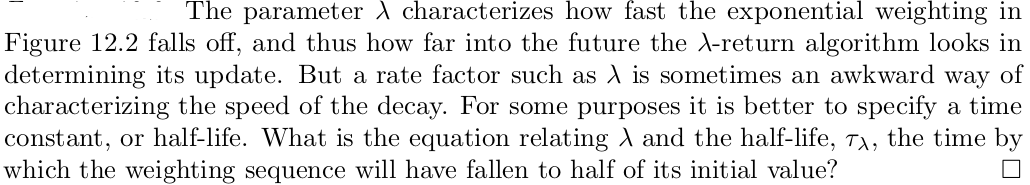
\includegraphics[scale=0.9]{exercise_12_2q}

    \subsection*{Answer}

    \noindent Half of initial weighting sequence:
    \noindent $ \frac{(1-\lambda)}{2} $

    \noindent Weighting sequence at time $t+m$:
    \noindent $ (1-\lambda) \lambda^m $

    \noindent Then by definition:
    \noindent $ (1-\lambda) \lambda^m = \frac{(1-\lambda)}{2} $

    \noindent $ \lambda^m = \frac{1}{2} $

    \noindent $ m = \log_{\lambda} \frac{1}{2} = - \log_{\lambda} 2 = \frac{\ln 2}{\ln \lambda}$

    \noindent The actual time step is:

    \noindent $ \tau_{\lambda} = t + m = t + \frac{\ln 2}{\ln \lambda} $


    \subsection{Question}

    Some insight into how $ TD(\lambda) $ can closely approximate the offline $\lambda$-return algorithm can be gained by seeing that the latter’s error term (in brackets in (12.4)) can be written as the sum of TD errors (12.6) for a single fixed w.
    Show this, following the pattern of (6.6), and using the recursive relationship for the $\lambda$-return you obtained in Exercise 12.1.

    \subsection*{Answer}

    \noindent Error term in (12.4) ($ w_{t+1} = w_t + \alpha [G_{t}^{\lambda} - \hat{v}(S_t, w_t)]\Delta \hat{v}(S_t, w_t)  $):

    \noindent $ G_{t}^{\lambda} - \hat{v}(S_t, w_t) $

    \hfill \break
    \noindent TD error (12.6):

    \noindent $ \delta_t = R_{t+1} + \gamma \hat{v}(S_{t+1}, w_t) - \hat{v}(S_t,w_t) $

    \hfill \break
    \noindent Recursive relationship for the $\lambda$-return obtained in Exercise 12.1:

    \noindent $ G_{t}^\lambda =  R_{t+1} + (1-\lambda) \gamma \hat{v}(S_{t+1},w_{t}) +  \gamma \lambda G_{t+1}^\lambda $

    \hfill \break
    \noindent Following the pattern of (6.6):

    \noindent $ G_{t}^{\lambda} - \hat{v}(S_t, w_t) = R_{t+1} + (1-\lambda) \gamma \hat{v}(S_{t+1},w_{t}) +  \gamma \lambda G_{t+1}^\lambda - \hat{v}(S_t, w_t) $

    \noindent $ G_{t}^{\lambda} - \hat{v}(S_t, w_t) = R_{t+1}  + (1-\lambda) \gamma \hat{v}(S_{t+1},w_{t}) +  \gamma \lambda G_{t+1}^\lambda - \hat{v}(S_t, w_t) - \gamma \hat{v}(S_{t+1}, w_t) + \gamma \hat{v}(S_{t+1}, w_t) $

    \noindent $ G_{t}^{\lambda} - \hat{v}(S_t, w_t) = \delta_{t} + (1-\lambda) \gamma \hat{v}(S_{t+1},w_{t}) +  \gamma \lambda G_{t+1}^\lambda - \gamma \hat{v}(S_{t+1}, w_t) $

    \noindent $ G_{t}^{\lambda} - \hat{v}(S_t, w_t) = \delta_{t} -\lambda \gamma \hat{v}(S_{t+1},w_{t}) +  \gamma \lambda G_{t+1}^\lambda $

    \noindent $ G_{t}^{\lambda} - \hat{v}(S_t, w_t) = \delta_{t} -\lambda \gamma \hat{v}(S_{t+1},w_{t}) +  \gamma \lambda [R_{t+2} + (1-\lambda) \gamma \hat{v}(S_{t+2},w_{t+1}) +  \gamma \lambda G_{t+2}^\lambda + \gamma \hat{v}(S_{t+2},w_{t+1}) - \gamma \hat{v}(S_{t+2},w_{t+1})] $

    \noindent $ G_{t}^{\lambda} - \hat{v}(S_t, w_t) = \delta_{t} +  \gamma \lambda [ \delta_{t+1} + (1-\lambda) \gamma \hat{v}(S_{t+2},w_{t+1}) +  \gamma \lambda G_{t+2}^\lambda - \gamma \hat{v}(S_{t+2},w_{t+1})] $

    \noindent $ G_{t}^{\lambda} - \hat{v}(S_t, w_t) = \delta_{t} +  \gamma \lambda [ \delta_{t+1} -\lambda \gamma \hat{v}(S_{t+2},w_{t+1}) +  \gamma \lambda G_{t+2}^\lambda] $

    \hfill \break
    \noindent for t = T-1, the inner-most expression will be:

    \noindent $ \delta_{T-2} - \gamma \lambda \hat{v}(S_{T-1}, w_{T-2}) + \gamma \lambda G_{T-1}^\lambda = \delta_{T-2} - \gamma \lambda \hat{v}(S_{T-1}, w_{T-2}) + \gamma \lambda G_t $

    \noindent $ = \delta_{T-2} - \gamma \lambda \hat{v}(S_{T-1}, w_{T-2}) + \gamma \lambda (R_T + \gamma \hat{v}(S_{T}, w_{T-1}) ) $

    \noindent $ = \delta_{T-2} + \gamma \lambda (R_T + \gamma \hat{v}(S_{T}, w_{T-1}) - \hat{v}(S_{T-1}, w_{T-2}) ) $

    \noindent $ = \delta_{T-2} + \gamma \lambda \delta_{T-1} $

    \hfill \break
    \noindent Now we can write whole expression as a proper sum:

    \noindent $ G_{t}^{\lambda} - \hat{v}(S_t, w_t) = \sum_{k=t}^{T-1} (\lambda \gamma)^{(k-t)} \delta_{k} $

    \subsection{Question}

    Use your result from the preceding exercise to show that, if the weight updates over an episode were computed on each step but not actually used to change the weights (w remained fixed),
    then the sum of TD($\lambda$)’s weight updates would be the same as the sum of the offline $\lambda$-return algorithm’s updates.

    \subsection*{Answer}

    \noindent Equation 12.5:

    \noindent $ z_{-1} = 0 $

    \noindent $ z_{t} = \gamma \lambda z_{t-1} + \Delta \hat{v}(S_t, w_t) $ where $ 0 \le t \le T $

    \hfill \break
    \noindent Let's try to write as a sum:

    \noindent $ z_{t} = \gamma \lambda z_{t-1} + \Delta \hat{v}(S_t, w) $

    \noindent $ z_{t} = \gamma \lambda ( \gamma \lambda z_{t-2} + \Delta \hat{v}(S_{t-1}, w) ) + \Delta \hat{v}(S_t, w) $

    \noindent $ z_{t} = \sum_{k=0}^{t} (\gamma \lambda )^{k-t} \Delta \hat{v}(S_k, w) $


    \hfill \break
    \noindent Sum of TD($\lambda$)’s weight updates:

    \noindent $ \alpha \sum_{t=0}^{\inf} \delta_t z_t = \alpha \sum_{t=0}^{\inf} \delta_t \sum_{k=0}^{t} (\gamma \lambda )^{t-k} \Delta \hat{v}(S_k, w) $

    \hfill \break
    \noindent Expanding the sum:

    \noindent t=0 $ \alpha \delta_0 [(\gamma \lambda)^0 \Delta\hat{v}(S_0, w)] $

    \noindent t=1 $ \alpha \delta_1 [(\gamma \lambda)^1 \Delta\hat{v}(S_0, w) + (\gamma \lambda)^0 \Delta\hat{v}(S_1, w) ] $

    \noindent t=2 $ \alpha \delta_2 [(\gamma \lambda)^2 \Delta\hat{v}(S_0, w) + (\gamma \lambda)^1 \Delta\hat{v}(S_1, w) + (\gamma \lambda)^0 \Delta\hat{v}(S_2, w) ] $

    \noindent t=3 $ \alpha \delta_3 [(\gamma \lambda)^3 \Delta\hat{v}(S_0, w) + (\gamma \lambda)^2 \Delta\hat{v}(S_1, w) + (\gamma \lambda)^1 \Delta\hat{v}(S_2, w) + (\gamma \lambda)^0 \Delta\hat{v}(S_3, w) ] $

    \hfill \break
    \noindent Let's sum vertically:

    \noindent $s = S_0$ $ \alpha \Delta\hat{v}(S_0, w) \sum_{k=0}^{\inf} (\gamma \lambda)^{k} \delta_{k} $

    \noindent $s = S_1$ $ \alpha \Delta\hat{v}(S_1, w) \sum_{k=0}^{\inf} (\gamma \lambda)^{k} \delta_{k+1} $

    \noindent $s = S_2$ $ \alpha \Delta\hat{v}(S_2, w) \sum_{k=0}^{\inf} (\gamma \lambda)^{k} \delta_{k+2} $

    \noindent $s = S_3$ $ \alpha \Delta\hat{v}(S_3, w) \sum_{k=0}^{\inf} (\gamma \lambda)^{k} \delta_{k+3} $

    \hfill \break
    \noindent $  \alpha \sum_{t=0}^{\inf} \delta_t z_t =  \sum_{t=0}^{\inf} \Delta\hat{v}(S_t, w) \sum_{k=0}^{\inf} (\lambda \gamma)^k \delta_{k+t} $

    \hfill \break
    \noindent Start inner index k from t so that it is similar to result of question 12.3:

    \noindent $  \alpha \sum_{t=0}^{\inf} \delta_t z_t =  \sum_{t=0}^{\inf} \Delta\hat{v}(S_t, w) \sum_{k=t}^{\inf} (\lambda \gamma)^{k-t} \delta_{t} $


    \hfill \break
    \noindent Now we can use result of question 12.3

    \noindent $  \alpha \sum_{t=0}^{\inf} \delta_t z_t =  \sum_{t=0}^{\inf} \Delta\hat{v}(S_t, w) (G_{t}^{\lambda} - \hat{v}(S_t, w_t)) $




\end{document}


